\documentclass[letterpaper,11pt]{article}

\usepackage{graphicx}
\usepackage{multicol}
\usepackage{fullpage}
\usepackage{csquotes}
\usepackage[margin=0.5in,letterpaper]{geometry}
\setlength{\footskip}{15pt}
\setlength{\belowcaptionskip}{9pt}
\usepackage{floatflt}
\usepackage{xspace}
\usepackage[margin=1cm,skip=9pt]{caption}
\usepackage{censor}
\usepackage{ulem}
\linespread{0.95}
\def\degC{$^{\circ}$C }
\def\degf{$^{\circ}$F }
\def\vol #1 {{\bf #1}, $\;\;$}
\def\refer{\par\noindent\hangindent\parindent\hangafter1}


\title{\vspace{-2.0cm}Herzmann Family Redacted Christmas Letter 2019}
\author{Daryl Herzmann${}^1$, Elizabeth Herzmann${}^2$, Margaret 
Herzmann${}^3$,\\
Robert Herzmann${}^4$, AND Charlotte Herzmann${}^5$ \\
\it{${}^1$ Corresponding Author},
\it{${}^2$ Responsible Adult},
\it{${}^3$ Senior Child},
\it{${}^4$ Growing Boy},
\it{${}^5$ Terrible Two}}
\date{16 December 2019}

\makeatletter
\newenvironment{tablehere}
  {\def\@captype{table}}
  {}

\newenvironment{figurehere}
  {\def\@captype{figure}}
  {}
\makeatother

\newcommand{\Line}[0]{%
  \rule{0cm}{0cm}\\\hrule\rule{0cm}{0cm}%
}

%\addtolength{\textheight}{1.5in}

\begin{document}
\maketitle
\vspace{-0.75cm}
\begin{abstract}
Attrition prevailed once again this year, so welcome back to another installment
of our annual letter.  Last year's tome (Herzmann et al., 2018) was not properly
vetted and may have publicly released classified sources and methods.
Additionally, Daryl's mother's side of the family contains many Muellers 
and so we are likely related to \textit{Special Counsel Robert S. Mueller, III}.  
As such, this year's letter has been properly redacted before release.
\end{abstract}

\vspace{-0.5cm}
\Line
%\vspace{-0.5cm}

\begin{multicols}{2}

    
\section{Introduction} 

The size of our family was not modified this year and comprises Daryl
\enquote{Daryl} (41), Elizabeth \enquote{Liz} \censor{..},
Margaret \enquote{Maggie Moo} (6), Robert \enquote{Ro-Ro} (5), Charlotte
 \enquote{Charlie Burger} (2), and one cat with a dog's name of Snoopy (11). 
The family implementation plan calls for size stability going forward.  All
family members managed to stay out of jail this year, except \censor{.....}
who \blackout{disturbed the peace after watching} 
\textit{The Price is Right}. 

   
\subsection{Housing}

Our house, circa 1996 with an octagon window, remains located in the same
swank Ankeny, IA location.  The children have yet to destroy it. Our living
room painting of ducks flying needed moved to make space for more monthly
picture documentation of our children's development (Fig 1).  It remains to
be seen how far into the children's teenage years this will be permitted
to continue.

\begin{figurehere}
    \centering   
    \resizebox{.95\columnwidth}{!}{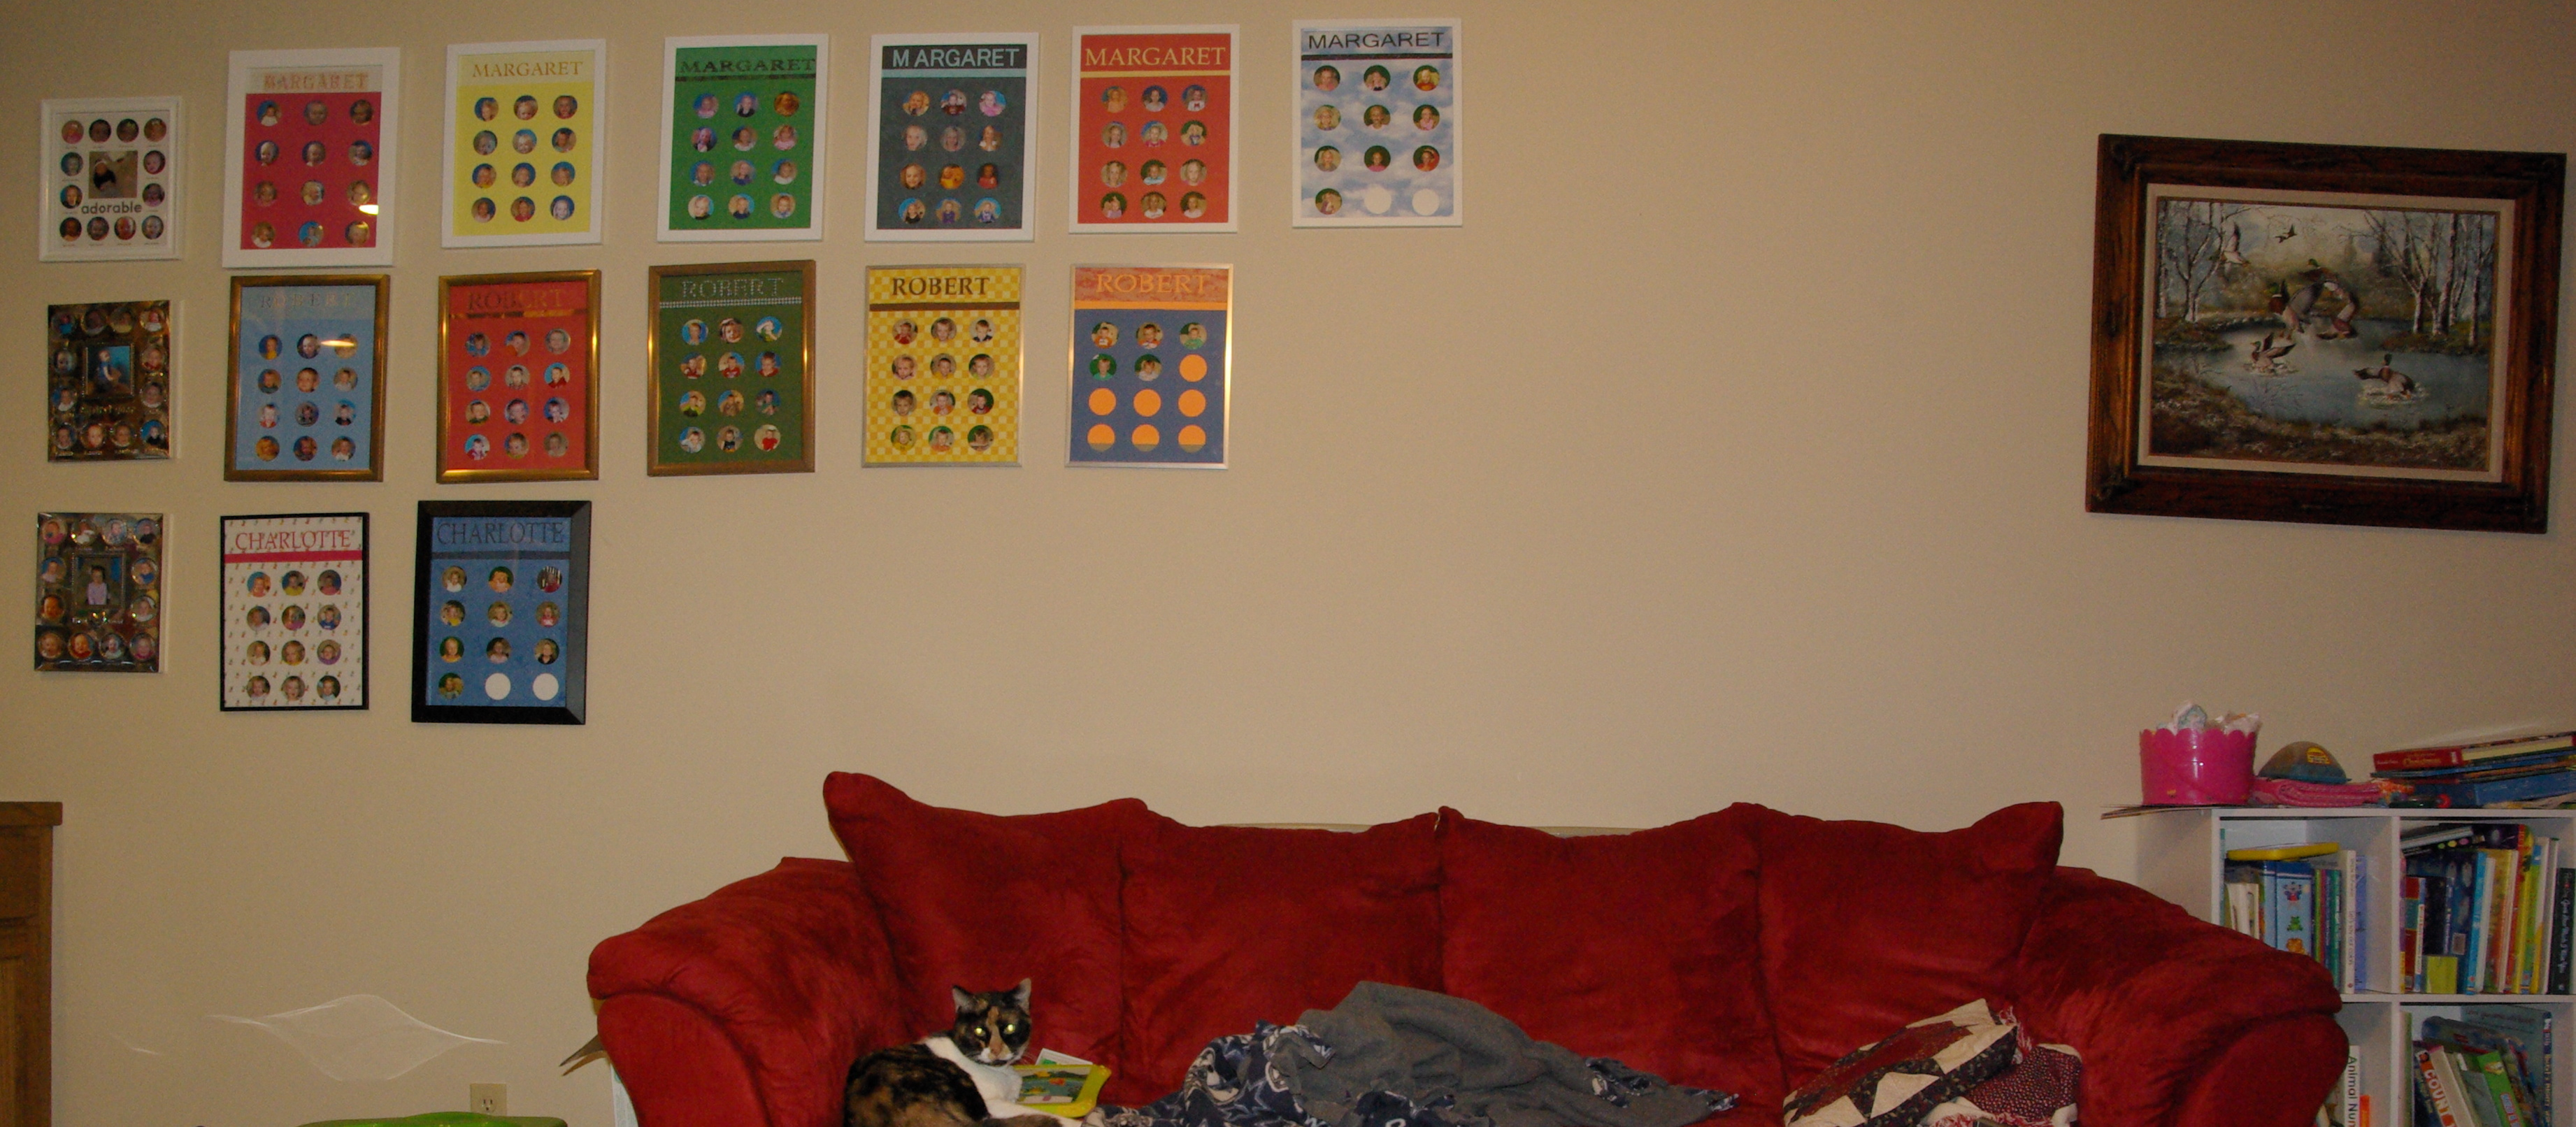
\includegraphics[angle=0]{plots/livingroom.eps}}
    \caption{Pedantic accounting of monthly development overseen by Snoopy the cat.}
   \end{figurehere}


\subsection{Employment}

Daryl continues to trek each day to Ames to work at Iowa State University as
he doesn't know any better.  He mostly writes software bugs each day 
related to soil erosion modeling, agronomic databasing, and weather data
collection.  He also monitor's the government's \sout{weather} modification program
named \censor{HAARP}, which spreads \blackout{blah and blah} from commercial
airplanes.

Liz continues to indoctrinate 8th grade youth at Southview Middle school
here in Ankeny.  This is her second year...

The children all seek opportunistic and transient employment to collect whatever
free change they suspect a nearby adult may have to offer.  Once the transaction
completes, they demand transportation to nearby store to spend it on items such
as \textit{Lunchables}, \textit{Legos}, and/or toys.

\section{Miss Charlotte}

Miss Charlotte's past year has lived up to the hype known as "Terrible Twos". She
has shown some interest in potty training, but is not there yet.  She insists that
momma be present for every activity.  She is a good child though and her language
skills 

\bigskip

\begin{figurehere}
 \centering   
 \resizebox{.95\columnwidth}{!}{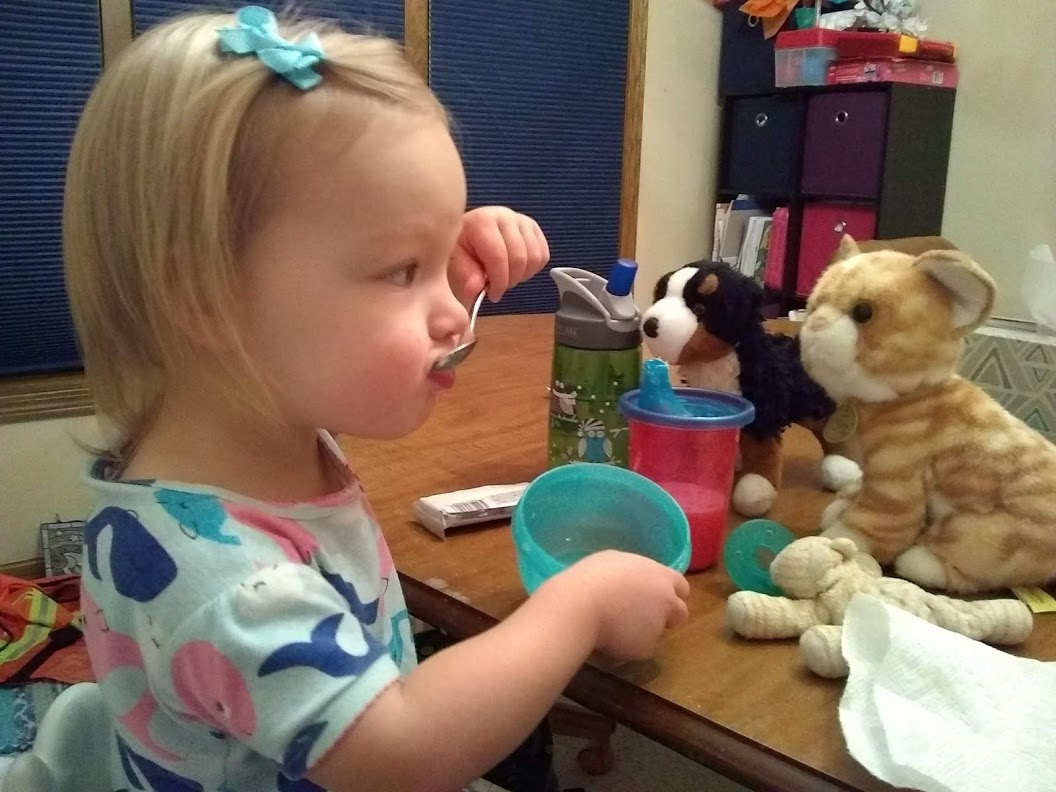
\includegraphics[angle=0]{plots/left.eps}}
 \caption{Charlotte eating breakfast with her left hand. Don't worry, will correct this.}
\end{figurehere}

\bigskip

Miss Charlotte loves to wrestle with anybody in the family willing and is already
roughing up Mr Robert more than he likes.  She is still a picky eater and prefers
to consume pancakes two at a time, one for each hand.

\section{Mr Robert}

Mr Robert is handful bundle of joy.  While his age is on the fence to be sent
to kindergarten in the fall, we are currently leaning toward enrolling him and
see what transpires. Mr Robert loves to play, be loud, and complain about his sisters,
parents, and the world in general being unfair to him.  He has breathtaking moments of
lucid deduction though, which are cherished memories for us.  For instance, he will
scream, while not wanting to go to bed, that if he stays up screaming that he will 
wake up grumpy tomorrow. The circular logic employed does not phase him.
He also seems to have an intrinsic understanding of
logistics and will make observations regarding inefficiencies of parental
work flows.

\section{Miss Maggie}

Miss Maggie is enjoying her first year of school at kindergarten and seems to be
a model student so far.  We were able to get her into our nearby elementary school,
which is a quick walk from our house.  She has surprised us with how quickly she
has picked up reading and doing math tasks.  After a quick foray into algebra,
a failed attempt was made at trigonometry.  She has shown recent interest in
the piano. Her favorite books include
\enquote{Fancy Nancy}, \enquote{WellieWishers\texttrademark}, and
\enquote{Berenstain Bears}.

We asked her if she wanted to contribute a paragraph to this article and she wanted
everyone to know that she likes snow and that is all.

\section{Summary}

We hoped you enjoyed reading this article, which was mailed with great care
as shown by Figure 3.  While tiring, life in our household is fun and full of
love.  The three children are such wonderful blessings and we are reminded daily of
how fortunate we are. 

\bigskip
\begin{figurehere}
 \centering   
 \resizebox{.95\columnwidth}{!}{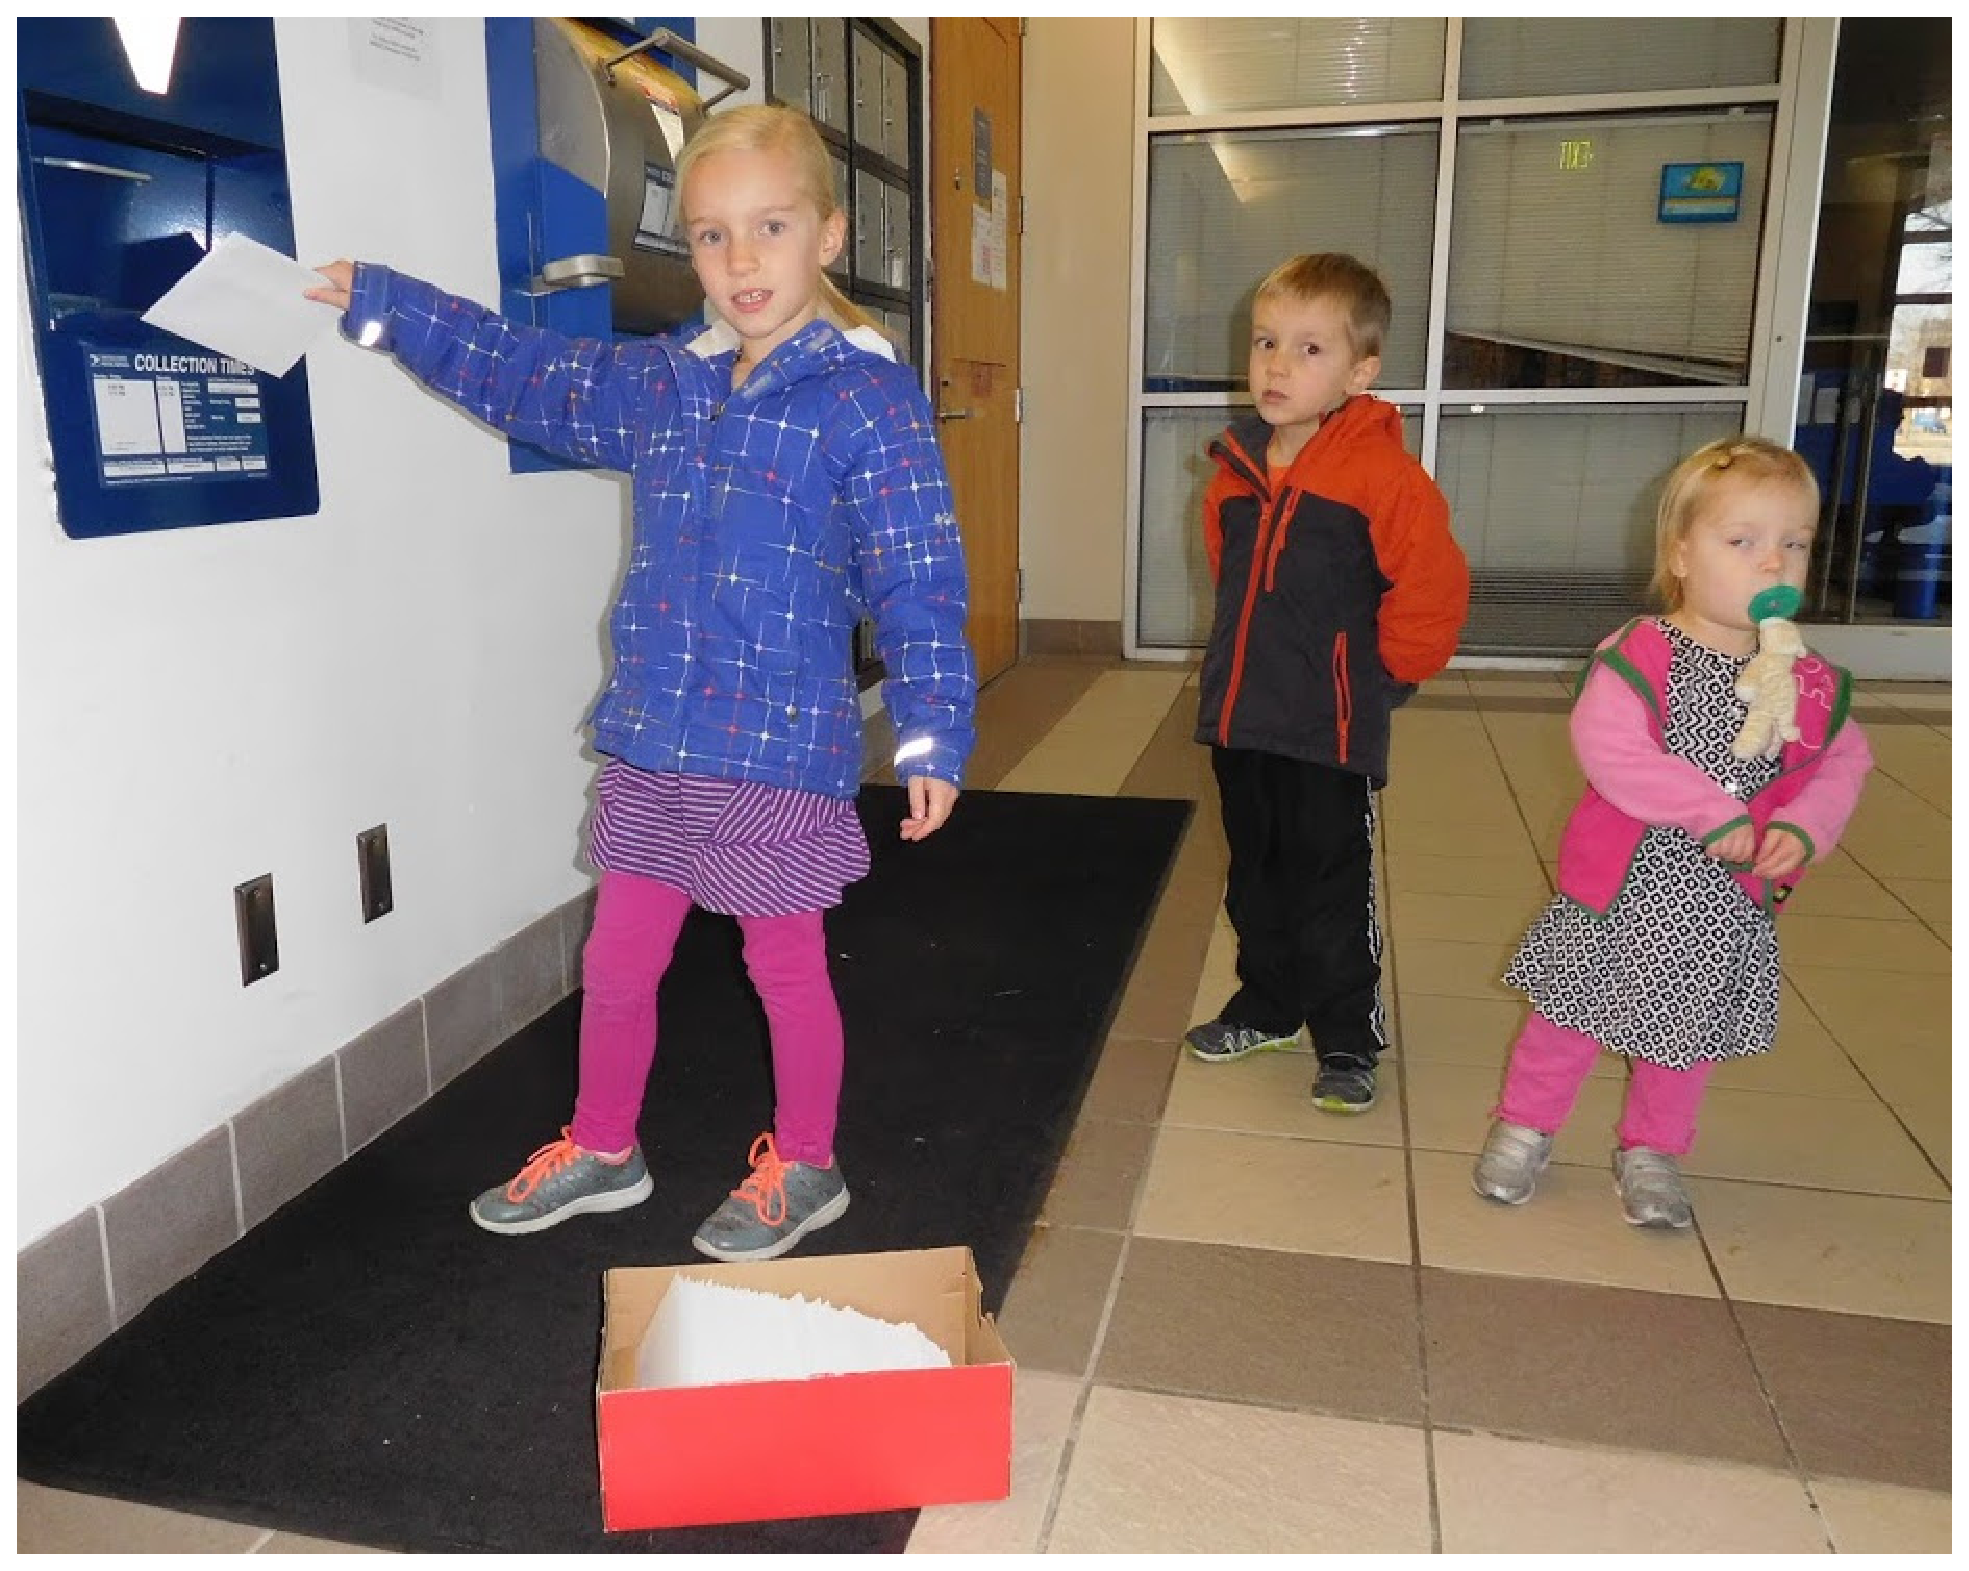
\includegraphics[angle=0]{plots/mail.eps}}
 \caption{The children delivering this year's letter to our local Amazon owned
 US Post Office. Miss Maggie thought it would be fun to place one letter at 
 a time into the mail box. \textsection \hspace{3pt} Kogen et al. 1990}
\end{figurehere}

\bigskip
  \emph{Acknowledgments} Our family wishes to thank you for the generous 
support, prayers, cards, gifts, and visits you have provided us in the past
year. With your continued support, this letter will be produced again
next year. Please note that the format chosen for this
correspondence was completely Daryl's idea and execution. Liz had marginal
editorial control. Full \LaTeX\xspace source can be found on Daryl's Github
page.

\section{References}

\refer Github, 2019: https://github.com/akrherz/me , visited 15 Dec 2019.
\refer Herzmann, Daryl E., et al. Herzmann Family Christmas Letter 2018.

\end{multicols}

\end{document}
